\begin{appendices}
%%% Appendix %%%
\section{User Manual}
For those who are interested in using the proposed class, the instruction is provided in this appendix.

\subsection{GitHub}
Git is an open-source version control system.  

Git is similar to other version control systems subversion, CVS.

For example \LaTeX{} template class you can clone git by url: http://bit.ly/2gt516q shown in Fig. \ref{fig:example0}

\begin{figure}[h]
  \centering
  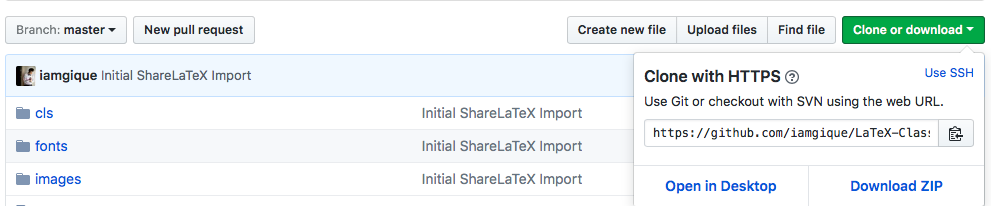
\includegraphics[width=5.6in]{example0.png}
  \caption{Clone Git repository.}
  \label{fig:example0}
\end{figure}

\subsection{Example source code to use}
After cloning repository at last version, please go to url: https://www.sharelatex.com then click New Project shown in Figure. \ref{fig:example1}

After that choose “Blank Project” shown in Figure. \ref{fig:example2} 

Input your project name then enter shown in Figure. \ref{fig:example3}

When create project success, please click “Upload” shown in Figure. \ref{fig:example4}

Select “Upload or Drag” file to dialog box. shown in Figure. \ref{fig:example5} and \ref{fig:example6}

Template class structure shown in Figure. \ref{fig:example7} when upload complete.

Select menu and then change compiler from “pdfLaTeX” to “XeLaTeX” and then click “Recompile” shown in Figure. \ref{fig:example8}

\begin{figure}[t!]
  \centering
  
\includegraphics[width=5.4in]{example1.png}
  \caption{New Project.}
  \label{fig:example1}
\end{figure}

\begin{figure}[t!]
  \centering
  
\includegraphics[width=2.4in]{example2.png}
  \caption{Choose Blank Project.}
  \label{fig:example2}
\end{figure}

\begin{figure}[t!]
  \centering
  
\includegraphics[width=5.4in]{example3.png}
  \caption{Input your project name.}
  \label{fig:example3}
\end{figure}

\begin{figure}[t!]
  \centering
  
\includegraphics[width=2.5in]{example4.png}
  \caption{Upload template class.}
  \label{fig:example4}
\end{figure}

\begin{figure}[t!]
  \centering
  
\includegraphics[width=4.4in]{example5.png}
  \caption{Upload or Drag file.}
  \label{fig:example5}
\end{figure}

\begin{figure}[t!]
  \centering
  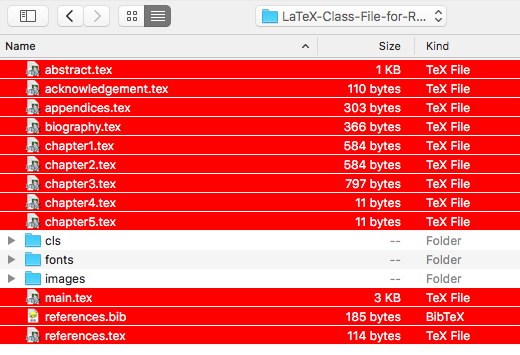
\includegraphics[width=4.0in]{example6.png}
  \caption{Upload process.}
  \label{fig:example6}
\end{figure}

\begin{figure}[t!]
  \centering
  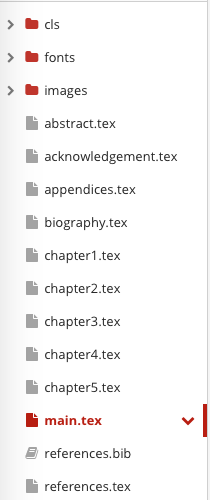
\includegraphics[width=2.0in]{example7.png}
  \caption{Template class structure.}
  \label{fig:example7}
\end{figure}

\begin{figure}[t]
  \centering
  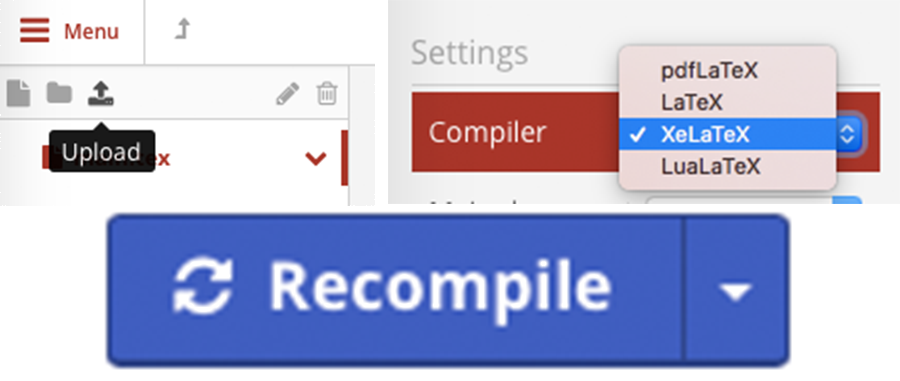
\includegraphics[width=4.0in]{example8.png}
  \caption{Change compiler and Recompile.}
  \label{fig:example8}
\end{figure}

\end{appendices}
\endappendices